\documentclass{ieeeaccess}
\usepackage{cite}
\usepackage{amsmath,amssymb,amsfonts}
\usepackage{algorithmic}
\usepackage{graphicx}
\usepackage{textcomp}
\usepackage{color}
\usepackage[normalem]{ulem}
\usepackage{environ}
\usepackage[font=footnotesize,labelfont=sf,textfont=sf]{subcaption}
\usepackage{multirow}

\usepackage[caption=false,font=footnotesize]{subfig}
\usepackage{booktabs}
\usepackage{wrapfig}

\definecolor{accessblue}{cmyk}{1,0.5,0,0}
\makeatletter
\long\def\@makecaption#1#2{
\ifx\@captype\ftype@table%
\begin{flushleft}
\vspace*{5pt}
\parbox{\columnwidth}{\vss{\color{accessblue}\tablecapheadfont #1. \ }\raggedright\tablecapfont#2\vss}%
\end{flushleft}
\else%
\begin{flushleft}
\vspace*{5pt}
\parbox{\columnwidth}{\vss{\color{accessblue}\figcapheadfont #1. \ }\raggedright\figcapfont#2\vss}%
\end{flushleft}
\fi}
\makeatother

\usepackage{bm}
\makeatletter
\AtBeginDocument{\DeclareMathVersion{bold}
\SetSymbolFont{operators}{bold}{T1}{times}{b}{n}
\SetSymbolFont{NewLetters}{bold}{T1}{times}{b}{it}
\SetMathAlphabet{\mathrm}{bold}{T1}{times}{b}{n}
\SetMathAlphabet{\mathit}{bold}{T1}{times}{b}{it}
\SetMathAlphabet{\mathbf}{bold}{T1}{times}{b}{n}
\SetMathAlphabet{\mathtt}{bold}{OT1}{pcr}{b}{n}
\SetSymbolFont{symbols}{bold}{OMS}{cmsy}{b}{n}
\renewcommand\boldmath{\@nomath\boldmath\mathversion{bold}}}
\makeatother

\def\BibTeX{{\rm B\kern-.05em{\sc i\kern-.025em b}\kern-.08em
    T\kern-.1667em\lower.7ex\hbox{E}\kern-.125emX}}

% Revision markup removed; macros no longer used.


%Your document starts from here ___________________________________________________
\begin{document}
\bstctlcite{IEEEexample:BSTcontrol}
\history{Date of publication xxxx 00, 0000, date of current version xxxx 00, 0000.}
\doi{10.1109/ACCESS.2024.0429000}

\title{Estimation of physical activity level of people \\in office environment by LiDAR sensor network}
\author{
    \uppercase{Wataru Sano}\authorrefmark{1},
    \uppercase{Koki Kizawa}\authorrefmark{1},
    \uppercase{Ken Kameoka}\authorrefmark{1},
    \uppercase{Ryusei Sugano}\authorrefmark{1}, \IEEEmembership{Graduate Student Member, IEEE},
    \uppercase{Ryoichi Shinkuma}\authorrefmark{1, 2}, \IEEEmembership{Senior Member, IEEE},
    \uppercase{Gabriele Trovato}\authorrefmark{1}, \IEEEmembership{Associate Member, IEEE}
}

\address[1]{Shibaura Institute of Technology, Tokyo, Japan}
\address[2]{Hyper Digital Twins Co., Ltd., Tokyo, Japan}

\tfootnote{This work was supported in part by JSPS KAKENHI, Japan, under Grant Nos. 23H00464 and 25H01124.}

\markboth
{K.Kizawa \headeretal: Estimation of physical activity level of people in office environment by LiDAR sensor network}
{K.Kizawa \headeretal: Estimation of physical activity level of people in office environment by LiDAR sensor network}

\corresp{Corresponding author: Wataru Sano (e-mail: al20104@shibaura-it.ac.jp).}


\begin{abstract}
  % 提案システムの目的
This paper proposes a system that estimates the activity levels of office workers using a light detection and ranging (LiDAR) sensor network.
% 点群の特徴抽出
Point-cloud data of individuals at work are captured by LiDAR and converted into numerical features.
% 機械学習による推論
Machine-learning models are employed to estimate the activity levels from the features.
\deleted{Activity level is defined as the degree of concentration during PC-based deskwork.}
\revised{Activity level is defined as a measure of learning efficiency during comprehension of meeting explanations and training content in offices.}
\deleted{Image-based and centroid-based features were extracted from point-cloud data.}
\revised{Image-based and centroid-based features are extracted from point-cloud data.}
% 評価実験
Evaluation experiments were conducted in office environments while participants watched learning videos.
% 活動レベルの評価
Activity indicators were derived from objective evaluation and subjective evaluation, and binary labels were generated using clustering for model evaluation.
% モデルの評価
Several models utilizing different feature types were developed and assessed against the binary labels.
% 結果
\deleted{The results demonstrate that three-dimensional features are effective for activity level estimation.}
\revised{Eight of the ten RF and XGBoost models exceeded a random-inference baseline of 0.5.}

\end{abstract}

\begin{keywords}
desk worker, office activity, light detection and ranging, point-cloud, temporal feature, machine-learning.
\end{keywords}

\titlepgskip=-21pt

\maketitle

\section{Introduction}
\label{sec:introduction}
%1st paragraph
%
Demand for monitoring physical activity in office environments has increased.
\deleted{Typical monitoring targets include posture changes during seated deskwork, hand movements during PC operation, and movements to use office equipment or communal areas.}
\revised{Typical monitoring targets include office activities such as posture changes during seated work, hand movements during PC operation, and movements to use office equipment or communal areas.}
%
Physical activity monitoring using smart office technologies has become socially growing awareness, aiming to improve employees' working conditions and enhance overall organizational performance \cite{PAPAGIANNIDIS2020102027}.
%

%2nd paragraph
%
Wearable devices, smart furniture, and RGB cameras have been used to monitor physical movements, stress, and office occupancy \cite{6627764,mozos2017stress,ouwerkerk2013wireless,krejcar2019smart,9216892,vlaovic2022smart,ayers2001monitoring,antonino2019office}.
Light detection and ranging (LiDAR) acquires 3D data for recognizing indoor movements of people and objects \cite{9795869,oka2021spatial,10159661}.
\deleted{Multiple LiDAR sensors can cover indoor spaces without blind spots \cite{oka2021spatial,10159661}.}
\revised{Multiple LiDAR sensors provide the following benefits \cite{oka2021spatial,10159661}.
The sensors cover indoor spaces without blind spots.
Integration of multi-view point-cloud data increases point density.
Multi-view integration captures the full surface of a person.}

%3rd paragraph
Zenonos et al.\ presented a mood-prediction system using wearable physiological data \cite{7457166}.
Yang et al.\ presented a multi-camera indoor tracking system \cite{4284740}.
Behera et al.\ presented a multi-camera surveillance system for indoor environments \cite{6409058}.
Zenonos et al.\ relied on wearable physiological sensors \cite{7457166}.
Yang et al.\ and Behera et al.\ relied on RGB cameras for person detection and tracking \cite{4284740,6409058}.
These sensing modalities share the burden or privacy concerns described above.
The aforementioned studies have the following challenges:
studies using wearable devices have not considered the discomfort and burden associated with wearing such devices, and contain potential privacy risk.

%4th paragraph
% 提案システム
This paper proposes a system that estimates activity levels of office workers from spatial features extracted from 3D point-cloud data.
%
\deleted{Activity level is defined as the degree of concentration during PC-based deskwork.}
  %
  \deleted{The activity level indicates whether a person is focused on the task or has lost concentration.}
\deleted{Concentration is assumed to accompany active movements that appear as dynamic patterns in LiDAR data.}
\revised{Activity level is defined as a measure of learning efficiency during comprehension of meeting explanations and training content in offices.}
%
\revised{Numerical features represent 3D characteristics of point-cloud data, such as the spatial center of mass.}
%
Point-cloud data were collected during multiple short video viewing using multiple LiDAR sensors.
%
Activity indicators were obtained from objective and subjective evaluations of the video content.
%
Clustering was applied to the indicators to generate binary labels.
%
\deleted{Numerical features represent 3D characteristics of point-cloud data, such as the spatial center of mass.}
%
Binary labels were generated on the basis of the consistency of clustered activity indicators among dataset pairs.
%
Multiple models using different feature types were constructed, and their accuracy was evaluated using the binary labels.

%5th paragraph
\deleted{We previously presented an edge computing system that estimates activity levels of people working in office environments using a LiDAR sensor network \cite{kizawa2023estimation}.}
\revised{We previously presented an edge computing system that estimates physical activities of people in offices using a LiDAR sensor network \cite{kizawa2023estimation}.}
\deleted{Differently from the previous study, our study addresses estimation models using multiple features.
The previous study characterized the collected point-cloud data using a single method and a statistical model as the estimation model and using linear correlation as the evaluation metric.}
\revised{The differences between this study and the previous study are as follows.
The previous study estimated physical activities represented by a quantitative indicator from a single motion feature using a statistical model.
This study estimates activity levels represented by subjective and quantitative indicators from multiple features using machine-learning models.}
% A previous edge computing system used a single feature extraction method and a statistical model with linear correlation as the evaluation metric \cite{kizawa2023estimation}.
% The present study addresses estimation models using multiple features.
% The previous study extracted a single statistical feature from point-cloud frame similarity and evaluated estimation using linear correlation \cite{kizawa2023estimation}.

%6th paragraph
Section~\ref{sec:related-works} reviews related works.
Section~\ref{sec:proposed-system} describes the system model, feature extraction, and labeling.
Section~\ref{sec:evaluation} explains the experimental setup and machine-learning models.
Section~\ref{sec:evaluation-result} presents the evaluation results.
Section~\ref{sec:conclusion} concludes the paper.


\section{Related works}
\label{sec:related-works}
\subsection{Other applications of LiDAR-sensor networks}
LiDAR sensor networks have been applied to autonomous driving, land-cover classification, and smart-city traffic monitoring \cite{9090850,Sun_2021_CVPR,8846588,8737958}.
The present study applies LiDAR sensor network technology to office environments for activity level estimation.
Yan et al.\ presented LMRoadNet for autonomous-driving road perception \cite{9090850}.
Sun et al.\ presented RSN for LiDAR-based 3D object detection \cite{Sun_2021_CVPR}.
Yu et al.\ presented a hybrid capsule network for land-cover classification \cite{8846588}.
Lv et al.\ presented LiDAR-enhanced connected infrastructure for smart-city traffic \cite{8737958}.
Prior LiDAR applications target outdoor or infrastructure-scale sensing.
Office deskwork requires non-contact estimation of subtle upper-body movements at desk scale.


\subsection{Study on physical activity in offices}
Physical activity in office environments is considered a critical factor in maintaining employee health and productivity \cite{PAPAGIANNIDIS2020102027}.
Existing studies assessed office activity levels through surveys and external factors \cite{RONGEN2013406,ALHORR2016369,DISHMAN1998344,de2005effect}.
The present study estimates activity levels from 3D features extracted from point-cloud data.
Rongen et al.\ reported small overall effects of workplace health promotion programs and emphasized the need for high-quality randomized controlled trials \cite{RONGEN2013406}.Al Horr et al.\ confirmed that indoor environmental quality factors significantly affect occupant productivity \cite{ALHORR2016369}.
Dishman et al.\ found limited statistically significant effects from workplace physical-activity interventions and noted low scientific quality in many studies \cite{DISHMAN1998344}.
Nooijen et al.\ identified habitual sitting as a major barrier to reducing sedentary behavior \cite{de2005effect}.
Survey-based and environmental-factor approaches do not capture individual deskwork movements during task execution.



\section{Proposed system}
\label{sec:proposed-system}
\subsection{System model}
\label{sec:system-model}
\begin{figure}[t]
  \centerline{\includegraphics[width=\linewidth]{img/system_model.png}}
  \caption{System model}
  \label{systemmodel}
\end{figure}

Fig.~\ref{systemmodel} shows a system model of the proposed system.
The phase of the proposed system switches between training and estimation.

Each 3D-sensor device consists of a LiDAR unit and an edge device with a converter, filter, and transmitter.
\deleted{The edge computer consists of a receiver and a merger \cite{9789786}.}
\revised{We adopt the multi-sensor filtering and merging scheme of Akiyama et al. \cite{9789786} for point-cloud acquisition.
The edge computer consists of a receiver and a merger.}
The user device consists of an interface and a capturer for activity level indicators.
\deleted{In the training phase, the edge server additionally consists ofa feature extractor, feature storage, a label creator, and a model constructor.}
\revised{In the training phase, the cloud server additionally consists of a feature extractor, feature storage, a label creator, and a model constructor.}
\deleted{LiDAR units acquire 3D stream data.}
\revised{LiDAR units acquire point-cloud data.}
\deleted{Edge devices convert the stream data into point-cloud data, apply filtering, and transmit the data to the edge computer.}
\revised{Edge devices apply filtering and transmit the data to the edge computer.}
\revised{Filtering reduces the volume of point-cloud data transmitted to the edge computer \cite{9789786}.}
The merger integrates point-cloud data from multiple sensors.
The feature extractor generates numerical features from the integrated data.
The label creator converts activity level indicators into categorical labels.
The model constructor builds a machine-learning model from the features and labels and stores it in the model database (DB).
\deleted{In the estimation phase, the edge server includes a feature extractor and an estimator.}
\revised{In the estimation phase, the cloud server includes a feature extractor and an estimator.}
The estimator applies the stored model to the generated features.
The user device and label creator are used only in the training phase to acquire activity level indicators and categorical labels.
The estimation phase omits the user device.
Point-cloud data flow is identical in both phases up to feature extraction.


\subsection{Methodology}
\label{sec:methodology}
Point-cloud data obtained from 3D-sensors consist of sets of 3D coordinates without individual point characteristics.
The number of frames and frame duration vary across datasets.
Target-object regions are extracted and converted into statistical features as described in Section~\ref{sec:feature-creation}.
Methods for identifying regions in 3D space are beyond the scope of the paper.
Activity levels are captured as multiple numerical indicators.
Contributors are grouped on the basis of the indicators and assigned labels as described in Section~\ref{sec:labeling}.
The features are evaluated on the basis of the assigned labels.
Statistical features are derived from datasets with varying frame counts and frame durations after target-object region extraction.


\subsection{Procedure}
\label{sec:procedure}
\subsubsection{Sensing}
\label{sec:sensing}
\deleted{3D stream data are acquired and converted into point-cloud data represented as sets of 3D coordinates.}
\revised{Point-cloud data are acquired as Cartesian coordinates.}
Point-cloud data from each device are integrated on the basis of timestamps and coordinates.


\subsubsection{Feature creation}
\label{sec:feature-creation}
\begin{figure}[t]
  \centerline{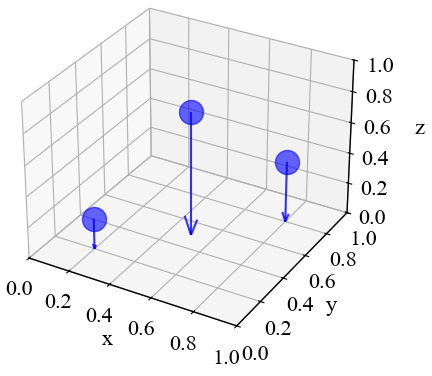
\includegraphics[width=\linewidth]{img/3d.png}}
  \caption{Projection of 3D coordinates}
  \label{trans3dto2d}
\end{figure}

Image-based feature modeling generates image arrays from time-series point-cloud frames and converts similarity changes between the arrays into statistics \cite{kizawa2023estimation}.
Overall physical movement is assumed to affect activity levels through changes in frame similarity.
\revised{Comparison of two point clouds requires point correspondence \cite{pomerleau2015review}.
Raw point-cloud frames do not provide the correspondence.
Frame-to-frame movement is not uniquely defined without the correspondence.
Orthogonal projection maps 3D occupancy onto a fixed 2D grid.}
For each frame, 3D point-cloud data are projected onto planes formed by pairs of the three coordinates ($x$, $y$, and $z$), as shown in Fig.~\ref{trans3dto2d}.
The projection is applied on all three axes for all frames.
Each 3D frame is converted into a 2D image to form a time-series 2D pixel array referred to as a `video frame'.
Frame-to-frame similarity is measured using zero-mean normalized cross-correlation (ZNCC) \cite{chen2020self,NAKHMANI2013315}.
ZNCC is computed between consecutive frames for the 1st to $I-1$-th frames, where $I$ is the number of frames.
The 50th and 90th percentile values of the ZNCC distribution are extracted as numerical features.
The 50th percentile value reflects the central tendency of the ZNCC distribution with minimal outlier influence.
The 90th percentile value captures upper-range similarity changes not represented by the central tendency alone.

Centroid feature modeling converts a head region of time-series point-cloud data into statistics of center-of-gravity changes.
Head movement is assumed to affect activity levels through center-of-gravity changes.
A head region is defined from 3D coordinates in an initial frame and extracted from all frames.
The sum of each coordinate in the head region is calculated for each frame.
Each frame is represented as a set of $n$ points ($x_{i}$, $y_{i}$, $z_{i}$) in 3D coordinate space.
The coordinate sums are defined as $X=\sum_{i=1}^{n}x_{i}$, $Y=\sum_{i=1}^{n}y_{i}$, and $Z=\sum_{i=1}^{n}z_{i}$.
The center of gravity $G_{j}$ for each frame up to $I$ is $G_{j}=(X/n, Y/n, Z/n)$, where $j$ is the frame number from the 1st to the $I$-th frame.
The central point $C$ of the center of gravity of all frames is $C=\frac{1}{I}\sum_{j=1}^{I}G_{j}$.
The difference between $C$ and $G_{j}$ is represented as Euclidean distance \cite{blais1995registering}.
The 50th and 90th percentile values of the center-of-gravity difference distribution are extracted as numerical features.


\subsubsection{Labeling}
\label{sec:labeling}
Numerical indicators of activity levels are normalized.
Participants are grouped on the basis of the indicators and assigned labels according to their groups.


\subsubsection{Model construction}
\label{sec:model-creation}
Activity levels are estimated using machine-learning models with multivariate feature inputs.
Feature-modeled point-cloud data serve as input and activity level labels serve as output.
Feature importance is extracted to analyze the impact of each feature on activity levels.



\section{Description of evaluation}
\label{sec:evaluation}
\subsection{Overview}
\label{sec:overview}
%
Evaluation experiments were conducted in office environments for PC-based deskwork.\footnote{The experiment was approved by the Ethics Committee of Shibaura Institute of Technology.}
Participants with similar professional backgrounds were recruited to reflect typical office group compositions of 10 to 15 members.
The scenario involved taking notes while viewing learning video content and taking a quiz afterward.
Activity levels were measured from subjective evaluation based on prior knowledge and comprehension, and objective evaluation based on quiz scores.
Data-acquisition experiments used multiple short learning videos.
\deleted{The learning-video scenario simulates sustained PC-based deskwork with note-taking and comprehension assessment.
Quiz scores provide objective indicators of content mastery.
Questionnaire responses provide subjective indicators of prior knowledge and comprehension.}
\revised{The learning-video scenario simulated sustained PC-based deskwork with note-taking and comprehension assessment.
Quiz scores provided objective indicators of content mastery.
Questionnaire responses provided subjective indicators of prior knowledge and comprehension.}


\subsection{Evaluation scenario}
\label{sec:scenario}
\deleted{PC-based deskwork is addressed among office tasks.
Activity levels are estimated by extracting specific regions and multiple dynamic features from point-cloud data of individuals engaged in deskwork.
The evaluation scenario involves relatively few complex movements common in office settings.
Point-cloud segmentation and feature-extraction methods from prior human activity recognition studies \cite{9861256,Qi_2017_CVPR} can extend the system to tasks beyond deskwork.
Deskwork involves relatively small movements compared with locomotion or equipment use.
The selected scenario enables controlled comparison of activity indicators and point-cloud features under identical task conditions.}
\revised{PC-based deskwork was addressed among office tasks.
Activity levels were estimated by extracting specific regions and multiple dynamic features from point-cloud data of individuals engaged in deskwork.
The evaluation scenario involved relatively few complex movements common in office settings.
Point-cloud segmentation and feature-extraction methods from prior human activity recognition studies could extend the system to tasks beyond deskwork \cite{9861256,Qi_2017_CVPR}.
Deskwork involved relatively small movements compared with locomotion or equipment use.
The selected scenario enabled controlled comparison of activity indicators and point-cloud features under identical task conditions.}


\subsection{Experimental system}
\label{sec:experiment-system}
\begin{figure}[t]
  \centerline{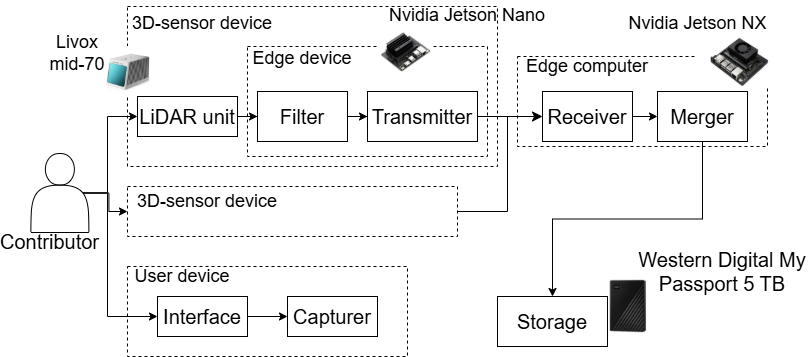
\includegraphics[width=\linewidth]{img/experiment_system.png}}
  \caption{Experiment system}
  \label{exp_system}
\end{figure}

\begin{figure}[t]
  \centerline{\includegraphics[width=\linewidth]{img/dyployment_site.png}}
  \caption{Experimental site}
  \label{exp_site}
\end{figure}

Fig.~\ref{exp_system} shows our experimental system based on Fig.~\ref{systemmodel}.
The experimental system consisted of multiple 3D-sensor devices, an edge computer, a user device, and storage.
\deleted{Point-cloud data from the sensors are filtered, transmitted, integrated on the basis of timestamps, and stored.}
\revised{Point-cloud data from the sensors were filtered, transmitted, integrated on the basis of timestamps, and stored.}
\deleted{The user device captures activity-level indicators.}
\revised{The user device captured activity level indicators.}
A Livox Mid-70 \cite{Mid70}, NVIDIA Jetson Nano \cite{Jetsonnano}, and NVIDIA Jetson Xavier NX \cite{JetsonNX} were used as the LiDAR unit, edge device, and edge computer, respectively.
Each contributor's laptop served as the user device.
\deleted{The evaluation verifies activity-level estimation from dynamic features extracted from 3D point-cloud data, without optimizing sensor placement or calibration \cite{9789786,10636133}.}
\revised{The evaluation verified activity level estimation from dynamic features extracted from 3D point-cloud data, without optimizing sensor placement or calibration \cite{9789786,10636133}.}
Akiyama et al.\ demonstrated that multiple LiDAR sensors can eliminate blind spots in indoor spaces \cite{9789786}.
\deleted{The present evaluation focuses on dynamic feature effectiveness rather than spatial calibration or sensor-placement optimization.}
\revised{The present evaluation focused on dynamic feature effectiveness rather than spatial calibration or sensor-placement optimization.}
Fig.~\ref{exp_site} shows the experimental site.
The experiment was conducted in lab room, located at the Toyosu Campus of Shibaura Institute of Technology in Koto-ku, Tokyo, Japan.
Each LiDAR unit was placed 1.0 m to the left and right of the center of the user-device keyboard, mounted at a height of 0.15 m using a tripod, tilted 10° horizontally with respect to the desk, and configured to operate at a sensing rate of 110 frames per second.


\subsection{Training dataset}
\label{sec:train-dataset}
\subsubsection{Experiment}
\label{sec:train-experiment}
%
Each participant used a personal laptop and followed steps from viewing a learning video to answering a quiz and questionnaire via Google Forms.
Notes could be referred to during the quiz.
The steps were repeated for each learning video.
Each participant received a learning video, notepad, quiz, and questionnaire.
Video viewing and note-taking started and stopped on an experimenter signal.
The quiz was completed before the questionnaire for each video.

%
The participants in the experiment were 37 students from Shibaura Institute of Technology.
  %
  Their ages ranged from 19 to 24.
  % %
  % The experiment was conducted from December 14th to 20th, 2022.
%
Three learning videos about structured query language (SQL) were examined~\cite{SQL}.
%
The durations of the videos were 206, 167, 116.
%
A quiz was created for each video, as shown in Table~\ref{quiz_train}.
  The quiz time limit was 300 s.
  A questionnaire rated understanding and prior knowledge on a scale from 1 to 5.


\subsubsection{Data acquisition by LiDAR}
\label{sec:train-lidar-data-acquisition}
%
Point-cloud data were acquired while participants viewed the videos.
110 datasets were obtained from 37 participants across three videos after removing one invalid dataset.
Feature extraction was applied using the image-based and centroid-based methods in Section~\ref{sec:feature-creation}.


\subsubsection{Data acquisition for labeling}
\label{sec:train-labeling}
Quiz scores were obtained as integer values from five one-point items per quiz.
Prior knowledge and understanding were obtained as responses to a two-item questionnaire. These responses were first converted to integer values on a scale from 0 to 4.
All values were then converted to real numbers between 0 and 1 for clustering.
Quiz scores and questionnaire responses were combined as numerical indicators for k-means clustering in Section~\ref{sec:train-evaluation}.


\subsubsection{Data processing for evaluation}
\label{sec:train-evaluation}
\begin{figure}[t]
  \centerline{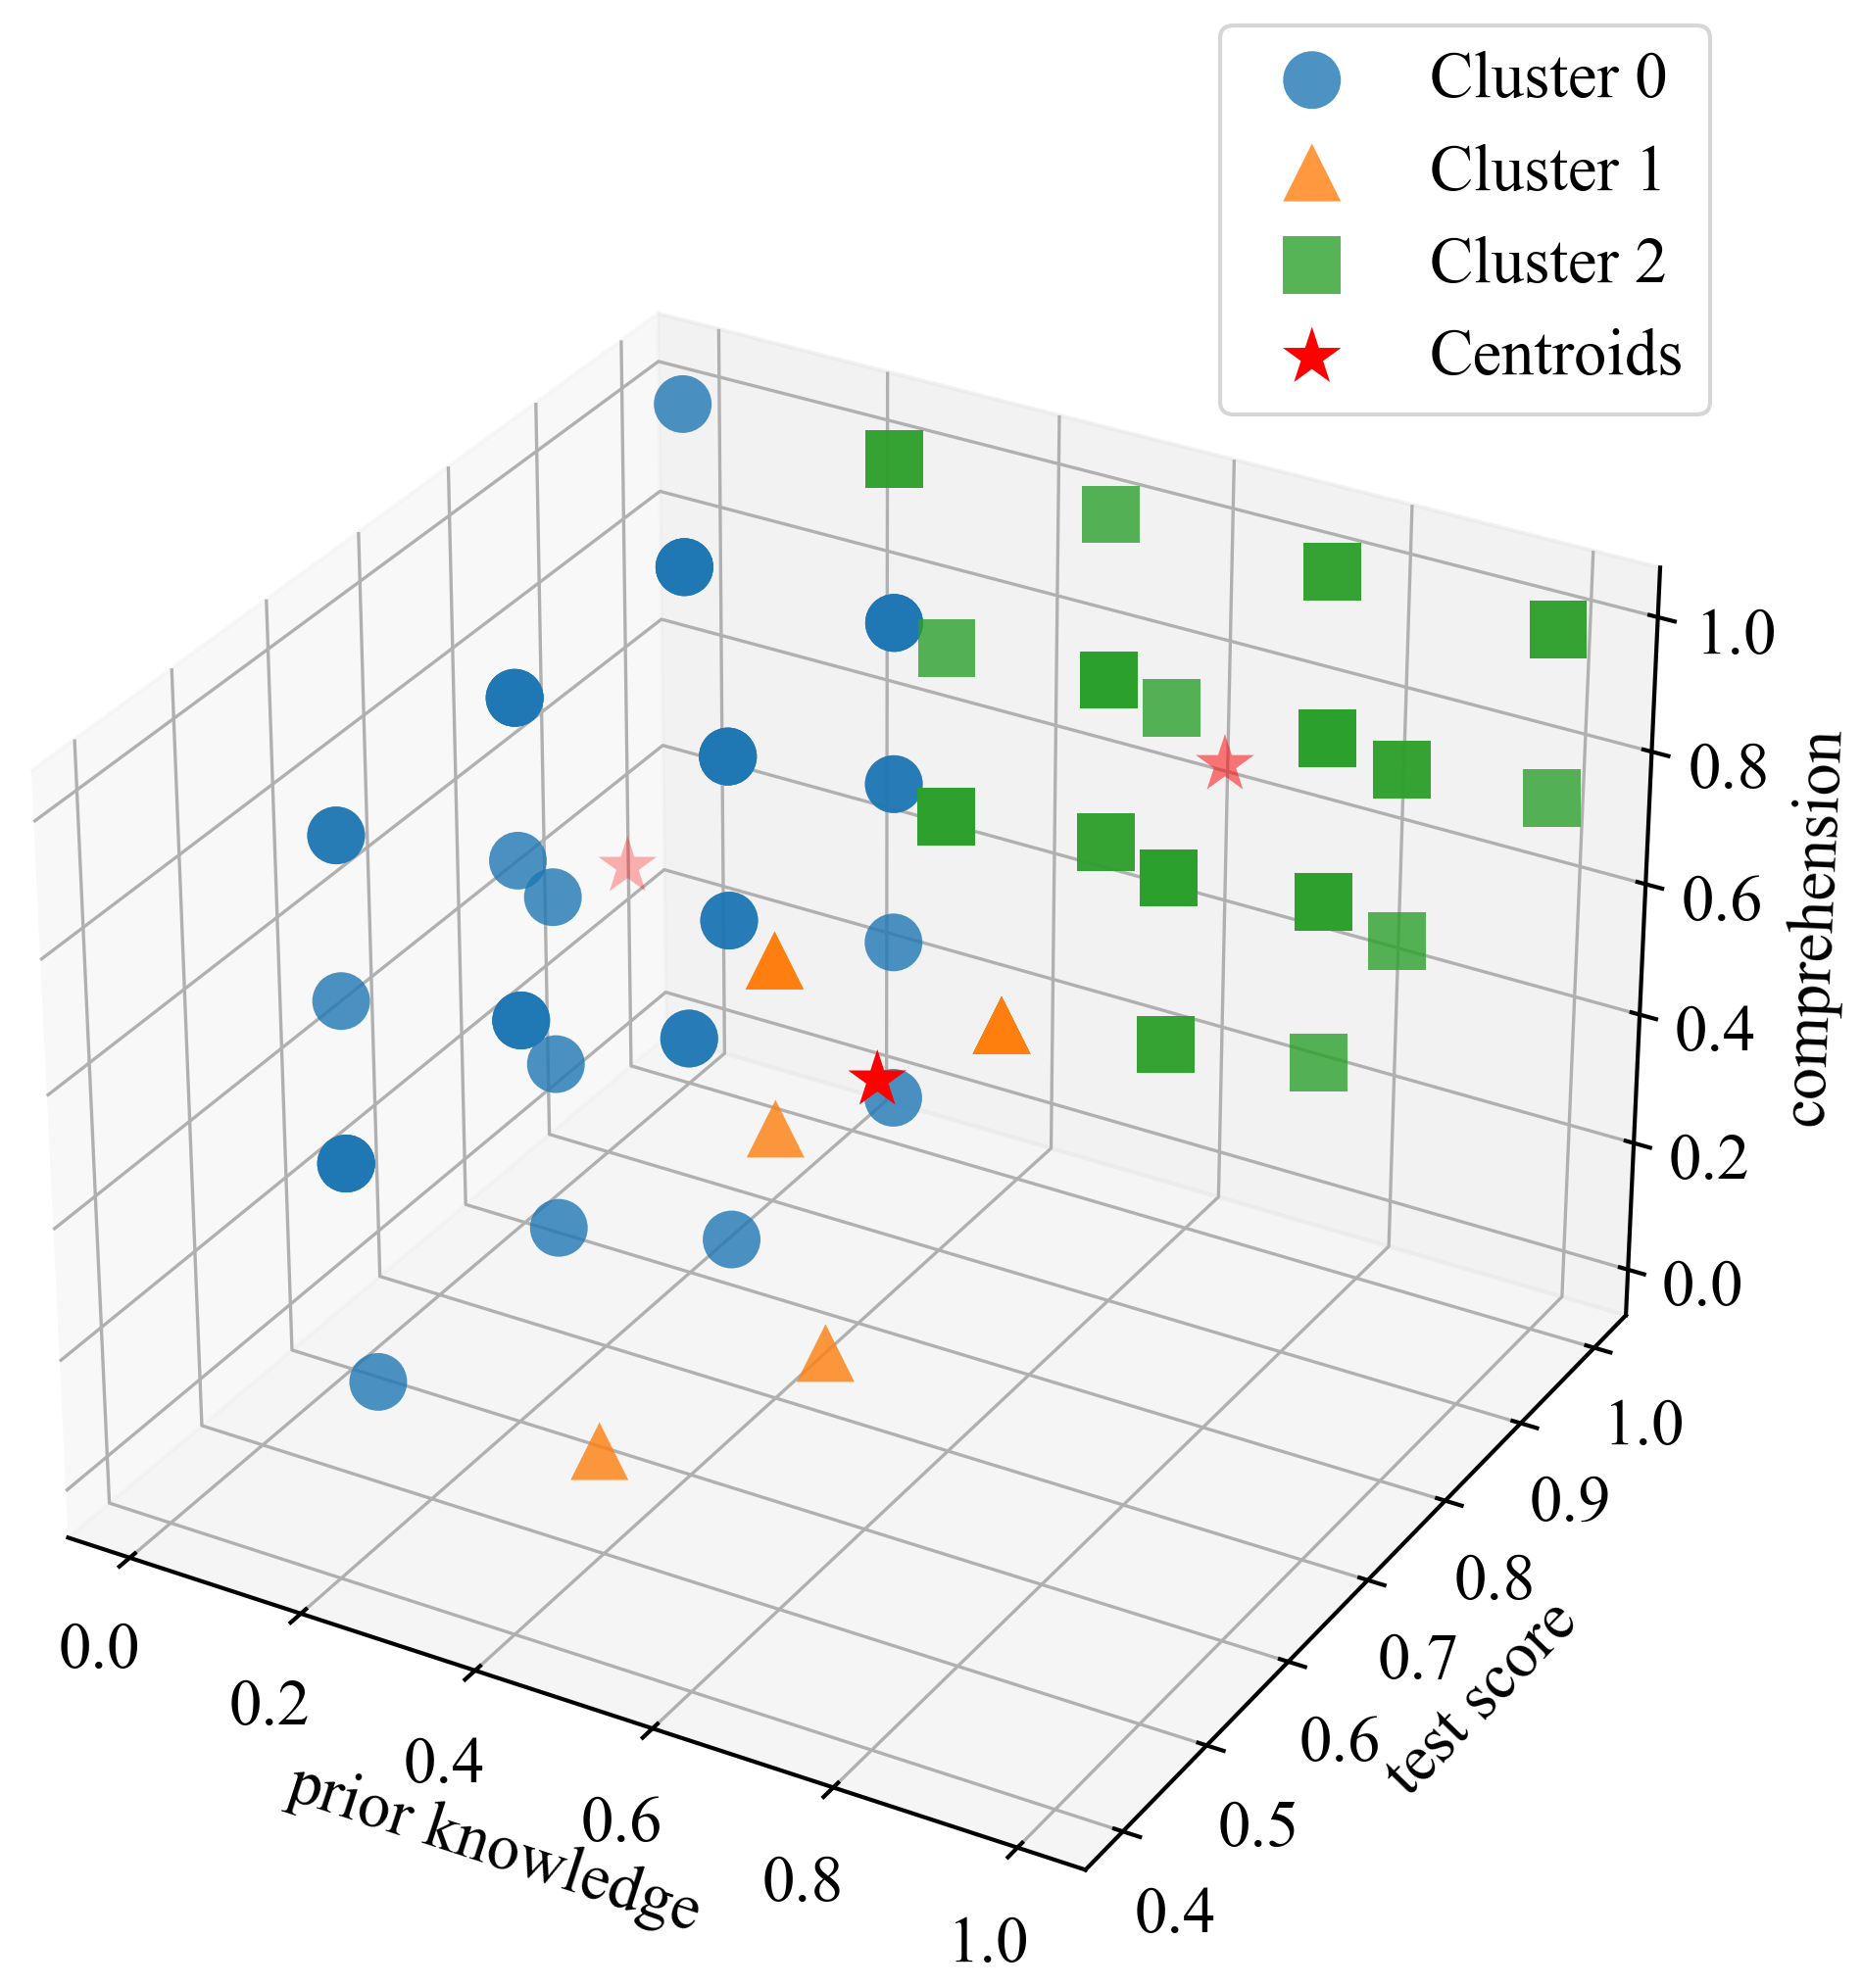
\includegraphics[width=\linewidth]{img/kmeans.png}}
  \caption{K-means result}
  \label{k-means_train}
\end{figure}

%1st paragraph
% 活動レベルの位置づけ
The activity levels were treated as a measure that integrates the subjective and objective perspectives.
  %
  The two indicators were converted into numerical labels by clustering.
  %
  The labels were defined as the group labels (GL).
    %
    GL represents the clustering results that capture multiple activity levels.
% k-meansの手順
K-means was used as a clustering method to split samples into $k$ groups \cite{krishna1999genetic}.
  %
  The number of clusters was set to $k=3$.
% k-meansの結果
Fig.~\ref{k-means_train} shows the clustering results.
% 点群データセットへのGLの割り当て
A GL cluster was assigned to each point-cloud dataset as an activity-level indicator.

%2nd paragraph
% データ拡張の実施
Data extension was performed to increase the available data samples.
\revised{Data extension compensated for the limited number of point-cloud datasets.
Public datasets combining video viewing and test-taking are unavailable.}
% データ拡張の方法
The datasets were extended by generating pairs of point-cloud datasets based on relational similarity~\cite{shinkuma2019relational}.
  % ペアの生成
  The point-cloud dataset pairs were formed from the $N=110$ point-cloud datasets ($\binom{N}{2}=5995$ pairs) without duplication.
  % ペアの特徴ベクトル間の絶対差分の計算
  The input features were computed as the element-wise absolute value of the difference between the feature vectors of each of the point-cloud dataset pairs.

%3rd paragraph
% MLの定義
Agreement and disagreement between the GL of the two datasets in each of the point-cloud datasets pairs are defined as matching labels (ML).
  % MLの形式
  ML is represented as a binary label.
\revised{Dataset pairs enabled supervised comparison of feature-vector differences between sessions with known GL relationships.}


\subsection{Machine-learning model}
\label{sec:machine-learning-model}
%
A machine-learning classification approach was used to estimate the activity levels of the participants.
%
Two machine-learning models were adopted: a random forest (RF) and an extreme gradient boosting (XGBoost) classifier \cite{ho1995random, 10.1145/2939672.2939785}.
%
Training and evaluation used short-video data.
RF and XGBoost were implemented using the scikit-learn application programming interface (API) \cite{pedregosa2011scikit,buitinck2013api}.
RF combines multiple decision trees and enables feature-importance evaluation during prediction \cite{ho1995random}.
XGBoost applies gradient boosting for high predictive accuracy \cite{10.1145/2939672.2939785}.
%
For each dataset pair, the element-wise absolute differences of point-cloud features were used as input.
  %
  ML derived from comparing the GL of the two datasets in each pair was used as output.
  %
  \deleted{The ML derived from GL is regarded as the ground truth, and the ML estimated by the model based on the features is regarded as the estimated result.}
  \revised{The ML derived from GL was regarded as the ground truth, and the ML estimated by the model based on the features was regarded as the estimated result.}
%
The dataset was randomly split into two parts: 80\% for training and 20\% for evaluation.
%
Hyperparameter tuning via grid search optimized the F1 score for each model \cite{10.5555/2188385.2188395}.
Predefined parameter sets for the number of estimators and maximum tree depth were explored for both RF and XGBoost.



\section{Evaluation result}
\label{sec:evaluation-result}
\subsection{Evaluation with short-video data}
\label{subsec:evaluation-short}
\begin{table}[!b]
  \centering
  \caption{Confusion matrices of RF models using short-video data. GT means ground truth, while ER means estimated result; diagonal components are correct.}
  \label{matrix_rf_train}

  \begin{tabular}{cc}
    \begin{subtable}{0.48\columnwidth} 
      \centering
      \caption{Image-50th}
      \label{matrix_rf_train_a}
      \scriptsize 
      \begin{tabular}{|lc|cc|}
        \hline
        \multicolumn{2}{|l|}{\multirow{2}{*}{}} & \multicolumn{2}{c|}{ER} \\ \cline{3-4}
        \multicolumn{2}{|l|}{} & \multicolumn{1}{c|}{0} & \multicolumn{1}{c|}{1} \\ \hline
        \multicolumn{1}{|c|}{\multirow{2}{*}{GT}} & 0 & \multicolumn{1}{c|}{98} & 30 \\ \cline{2-4}
        \multicolumn{1}{|c|}{} & 1 & \multicolumn{1}{c|}{59} & 23 \\ \hline
      \end{tabular}
      \vspace{5pt}
    \end{subtable}
    &
    \begin{subtable}{0.48\columnwidth}
      \centering
      \caption{Image-90th}
      \label{matrix_rf_train_b}
      \scriptsize
      \begin{tabular}{|lc|cc|}
        \hline
        \multicolumn{2}{|l|}{\multirow{2}{*}{}} & \multicolumn{2}{c|}{ER} \\ \cline{3-4}
        \multicolumn{2}{|l|}{} & \multicolumn{1}{c|}{0} & \multicolumn{1}{c|}{1} \\ \hline
        \multicolumn{1}{|c|}{\multirow{2}{*}{GT}} & 0 & \multicolumn{1}{c|}{72} & 56 \\ \cline{2-4}
        \multicolumn{1}{|c|}{} & 1 & \multicolumn{1}{c|}{42} & 40 \\ \hline
      \end{tabular}
      \vspace{5pt}
    \end{subtable}
    \\
    \begin{subtable}{0.48\columnwidth}
      \centering
      \caption{Centroid-50th}
      \label{matrix_rf_train_c}
      \scriptsize
      \begin{tabular}{|lc|cc|}
        \hline
        \multicolumn{2}{|l|}{\multirow{2}{*}{}} & \multicolumn{2}{c|}{ER} \\ \cline{3-4}
        \multicolumn{2}{|l|}{} & \multicolumn{1}{c|}{0} & \multicolumn{1}{c|}{1} \\ \hline
        \multicolumn{1}{|c|}{\multirow{2}{*}{GT}} & 0 & \multicolumn{1}{c|}{65} & 63 \\ \cline{2-4}
        \multicolumn{1}{|c|}{} & 1 & \multicolumn{1}{c|}{40} & 42 \\ \hline
      \end{tabular}
      \vspace{5pt}
    \end{subtable}
    &
    \begin{subtable}{0.48\columnwidth}
      \centering
      \caption{Centroid-90th}
      \label{matrix_rf_train_d}
      \scriptsize
      \begin{tabular}{|lc|cc|}
        \hline
        \multicolumn{2}{|l|}{\multirow{2}{*}{}} & \multicolumn{2}{c|}{ER} \\ \cline{3-4}
        \multicolumn{2}{|l|}{} & \multicolumn{1}{c|}{0} & \multicolumn{1}{c|}{1} \\ \hline
        \multicolumn{1}{|c|}{\multirow{2}{*}{GT}} & 0 & \multicolumn{1}{c|}{50} & 78 \\ \cline{2-4}
        \multicolumn{1}{|c|}{} & 1 & \multicolumn{1}{c|}{33} & 49 \\ \hline
      \end{tabular}
      \vspace{5pt}
    \end{subtable}
    \\
    \multicolumn{2}{c}{
    \begin{subtable}{0.48\columnwidth}
      \centering
      \caption{All features}
      \label{matrix_rf_train_e}
      \scriptsize
      \begin{tabular}{|lc|cc|}
        \hline
        \multicolumn{2}{|l|}{\multirow{2}{*}{}} & \multicolumn{2}{c|}{ER} \\ \cline{3-4}
        \multicolumn{2}{|l|}{} & \multicolumn{1}{c|}{0} & \multicolumn{1}{c|}{1} \\ \hline
        \multicolumn{1}{|c|}{\multirow{2}{*}{GT}} & 0 & \multicolumn{1}{c|}{78} & 50 \\ \cline{2-4}
        \multicolumn{1}{|c|}{} & 1 & \multicolumn{1}{c|}{42} & 40 \\ \hline
      \end{tabular}
      \vspace{5pt}
    \end{subtable}
    }
  \end{tabular}
\end{table}

\begin{table}[!b]
  \centering
  \caption{Accuracy using RF (short-video data)}
    \begin{tabular}{clll} \hline
      Feature         & Accuracy & FNR   & FPR   \\ \hline \hline
      Image-50th      & 0.576    & 0.720 & 0.234 \\
      Image-90th      & 0.533    & 0.512 & 0.438 \\
      Centroid-50th   & 0.510    & 0.488 & 0.492 \\
      Centroid-90th   & 0.471    & 0.402 & 0.609 \\
      All             & 0.562    & 0.512 & 0.391 \\ \hline
    \end{tabular}
  \label{result_rf_train}
\end{table}

\begin{table}[!b]
	\centering
	\caption{Feature importance of the RF model with all features as input}
	\begin{tabular}{clc}
		\hline
		Rank & Feature      & Feature Importance \\ \hline \hline
		1    & Centroid-50th  & 0.170            \\
		2    & Centroid-90th  & 0.167            \\
		3    & Image-90th (x) & 0.122            \\
		4    & Image-50th (z) & 0.114            \\
		5    & Image-90th (z) & 0.112            \\
		6    & Image-90th (y) & 0.111            \\
		7    & Image-50th (y) & 0.106            \\
		8    & Image-50th (x) & 0.097            \\ \hline
	\end{tabular}
	\label{feature_importance_rf}
\end{table}

\begin{table}[!b]
  \centering
  \caption{Confusion matrices of XGBoost models using short-video data. GT means ground truth, while ER means estimated result; diagonal components are correct.}
  \label{matrix_xg_train}

  \begin{tabular}{cc}
    \begin{subtable}{0.48\columnwidth}
      \centering
      \caption{Image-50th}
      \label{matrix_xg_train_a}
      \scriptsize
      \begin{tabular}{|lc|cc|}
        \hline
        \multicolumn{2}{|l|}{\multirow{2}{*}{}} & \multicolumn{2}{c|}{ER} \\ \cline{3-4}
        \multicolumn{2}{|l|}{} & \multicolumn{1}{c|}{0} & \multicolumn{1}{c|}{1} \\ \hline
        \multicolumn{1}{|c|}{\multirow{2}{*}{GT}} & 0 & \multicolumn{1}{c|}{86} & 42 \\ \cline{2-4}
        \multicolumn{1}{|c|}{} & 1 & \multicolumn{1}{c|}{55} & 27 \\ \hline
      \end{tabular}
      \vspace{5pt}
    \end{subtable}
    &
    \begin{subtable}{0.48\columnwidth}
      \centering
      \caption{Image-90th}
      \label{matrix_xg_train_b}
      \scriptsize
      \begin{tabular}{|lc|cc|}
        \hline
        \multicolumn{2}{|l|}{\multirow{2}{*}{}} & \multicolumn{2}{c|}{ER} \\ \cline{3-4}
        \multicolumn{2}{|l|}{} & \multicolumn{1}{c|}{0} & \multicolumn{1}{c|}{1} \\ \hline
        \multicolumn{1}{|c|}{\multirow{2}{*}{GT}} & 0 & \multicolumn{1}{c|}{67} & 61 \\ \cline{2-4}
        \multicolumn{1}{|c|}{} & 1 & \multicolumn{1}{c|}{46} & 36 \\ \hline
      \end{tabular}
      \vspace{5pt}
    \end{subtable}
    \\
    \begin{subtable}{0.48\columnwidth}
      \centering
      \caption{Centroid-50th}
      \label{matrix_xg_train_c}
      \scriptsize
      \begin{tabular}{|lc|cc|}
        \hline
        \multicolumn{2}{|l|}{\multirow{2}{*}{}} & \multicolumn{2}{c|}{ER} \\ \cline{3-4}
        \multicolumn{2}{|l|}{} & \multicolumn{1}{c|}{0} & \multicolumn{1}{c|}{1} \\ \hline
        \multicolumn{1}{|c|}{\multirow{2}{*}{GT}} & 0 & \multicolumn{1}{c|}{77} & 51 \\ \cline{2-4}
        \multicolumn{1}{|c|}{} & 1 & \multicolumn{1}{c|}{46} & 36 \\ \hline
      \end{tabular}
      \vspace{5pt}
    \end{subtable}
    &
    \begin{subtable}{0.48\columnwidth}
      \centering
      \caption{Centroid-90th}
      \label{matrix_xg_train_d}
      \scriptsize
      \begin{tabular}{|lc|cc|}
        \hline
        \multicolumn{2}{|l|}{\multirow{2}{*}{}} & \multicolumn{2}{c|}{ER} \\ \cline{3-4}
        \multicolumn{2}{|l|}{} & \multicolumn{1}{c|}{0} & \multicolumn{1}{c|}{1} \\ \hline
        \multicolumn{1}{|c|}{\multirow{2}{*}{GT}} & 0 & \multicolumn{1}{c|}{62} & 66 \\ \cline{2-4}
        \multicolumn{1}{|c|}{} & 1 & \multicolumn{1}{c|}{32} & 50 \\ \hline
      \end{tabular}
      \vspace{5pt}
    \end{subtable}
    \\
    \multicolumn{2}{c}{
    \begin{subtable}{0.48\columnwidth}
      \centering
      \caption{All features}
      \label{matrix_xg_train_e}
      \scriptsize
      \begin{tabular}{|lc|cc|}
        \hline
        \multicolumn{2}{|l|}{\multirow{2}{*}{}} & \multicolumn{2}{c|}{ER} \\ \cline{3-4}
        \multicolumn{2}{|l|}{} & \multicolumn{1}{c|}{0} & \multicolumn{1}{c|}{1} \\ \hline
        \multicolumn{1}{|c|}{\multirow{2}{*}{GT}} & 0 & \multicolumn{1}{c|}{81} & 47 \\ \cline{2-4}
        \multicolumn{1}{|c|}{} & 1 & \multicolumn{1}{c|}{39} & 43 \\ \hline
      \end{tabular}
      \vspace{5pt}
    \end{subtable}
    }
  \end{tabular}
\end{table}

\begin{table}[!b]
  \centering
	\caption{Accuracy using XGBoost (short-video data)}
		\begin{tabular}{clll} \hline
			Feature       & Accuracy & FNR   & FPR    \\ \hline \hline
			Image-50th    & 0.538    & 0.671 & 0.328  \\
			Image-90th    & 0.490    & 0.561 & 0.477  \\
			Centroid-50th & 0.538    & 0.561 & 0.398  \\
			Centroid-90th & 0.533    & 0.390 & 0.516  \\
			All           & 0.590    & 0.476 & 0.367  \\ \hline
		\end{tabular}
	\label{result_xg_train}
\end{table}

\begin{table}[!b]
	\centering
	\caption{Feature importance of the XGBoost model with all features as input}
	\begin{tabular}{clc}
		\hline
		Rank & Feature        & Feature Importance \\ \hline \hline
		1    & Centroid-50th  & 0.278              \\
		2    & Centroid-90th  & 0.166              \\
		3    & Image-50th (z) & 0.110              \\
		4    & Image-90th (z) & 0.094              \\
		5    & Image-50th (y) & 0.092              \\
		6    & Image-50th (x) & 0.089              \\
		7    & Image-90th (y) & 0.087              \\
		8    & Image-90th (x) & 0.083              \\ \hline
	\end{tabular}
	\label{feature_importance_xg}
\end{table}

%
\deleted{We present the result of the estimation using the short-video data described in Section \ref{sec:train-dataset}.}
\revised{The estimation results using the short-video data in Section~\ref{sec:train-dataset} are presented.}

\subsubsection{Results of RF evaluation}
Table~\ref{matrix_rf_train} shows confusion matrices of five RF models: four with a single feature and one with all features.
Table~\ref{result_rf_train} shows the evaluation metrics.
The model with image-based 50th percentile values achieved the highest accuracy.
The model with centroid 90th percentile values achieved the lowest false negative rate (FNR).
Table~\ref{feature_importance_rf} shows feature importance from the all-feature model (Table~\ref{matrix_rf_train_e}).
Centroid-50th and Centroid-90th showed the highest importance.
Centroid features reduced misclassifications among similar activity levels.
Image-based 50th percentile values achieved the highest accuracy among the five models.
Different 3D feature types provide complementary information for short video datasets.
For the RF model, the all-feature input did not outperform the image-based 50th percentile single-feature model in Table~\ref{result_rf_train}.
Image-based 50th percentile values showed moderate false negative rate (FNR) and slightly lower false positive rate (FPR) in Table~\ref{matrix_rf_train_a}.
Centroid 90th percentile values achieved the lowest FNR among the single-feature models.


\subsubsection{Results of XGBoost evaluation}
Table~\ref{matrix_xg_train} shows confusion matrices of five XGBoost models: four with a single feature and one with all features.
Table~\ref{result_xg_train} shows the evaluation metrics.
The all-feature model achieved the highest accuracy.
The model with centroid 90th percentile values achieved the lowest FNR.
Table~\ref{feature_importance_xg} shows feature importance from the all-feature model (Table~\ref{matrix_xg_train_e}).
Centroid-50th and Centroid-90th showed the highest importance.
Centroid features reduced misclassifications among similar activity levels.
A diverse set of three-dimensional features is effective for activity level estimation with XGBoost on short video datasets.
For the XGBoost model, the all-feature input outperformed every single-feature model in Table~\ref{result_xg_train}.
The contrast between RF and XGBoost indicates that complementary 3D features require an appropriate ensemble model to be fully exploited.



\subsection{Results analysis}
\label{sec:results-analysis}
Factors that may limit estimation accuracy are discussed.
Clustering stability is analyzed as a potential contributor to the limited improvement from multiple features.

% \begin{figure}[t]
% 	\centerline{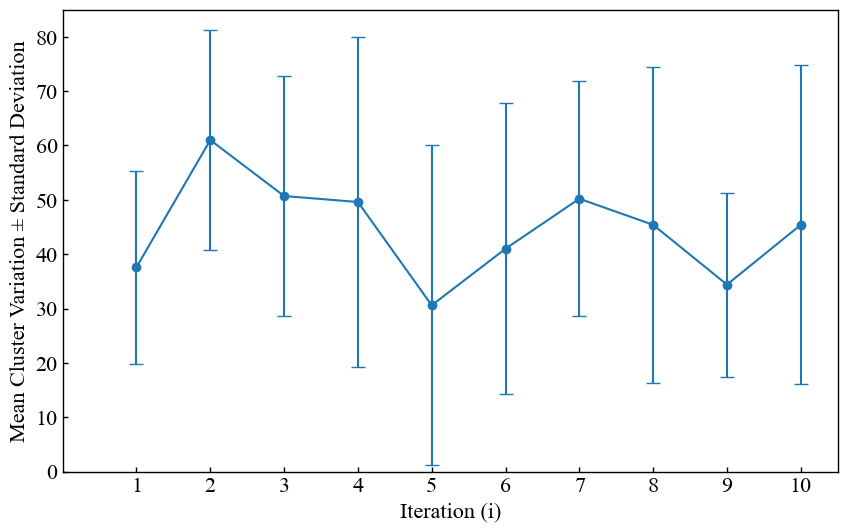
\includegraphics[width=\linewidth]{img/clustering.png}}
% 	\caption{Stability verification of cluster assignment for short video dataset}
% 	\label{fig:clustering-stability}
% \end{figure}

%
\revised{A random-inference baseline of 0.5 was used for binary classification.
Eight of the ten RF and XGBoost models exceeded the baseline on the short video dataset.
The result demonstrates that activity levels were estimated from point-cloud features.}

%
Section~\ref{subsec:evaluation-short} demonstrated that three-dimensional point-cloud features are effective for activity level estimation.
Clustering instability may partially explain the limited accuracy improvement from multiple features.
K-means clustering ($k$=3) was applied to the short video dataset as a baseline.
One sample was randomly removed and clustering was re-run 10 times per trial, repeated over 10 trials.
Cluster changes ranged from approximately 20 to 40 per trial.
Clustering instability is a contributing factor to the limited accuracy improvement from multiple features.
The XGBoost all-feature model achieved the highest accuracy in Section~\ref{subsec:evaluation-short}.
The accuracy gain over single-feature models remained limited.
A baseline clustering result was established with k-means ($k$=3) on the full dataset.
Mean and standard deviation of reassignment counts were computed across 10 trials of 10 removal-and-reclustering operations.


\subsubsection{Impact of clustering stability on estimation accuracy}
\begin{figure}[t]
	\centerline{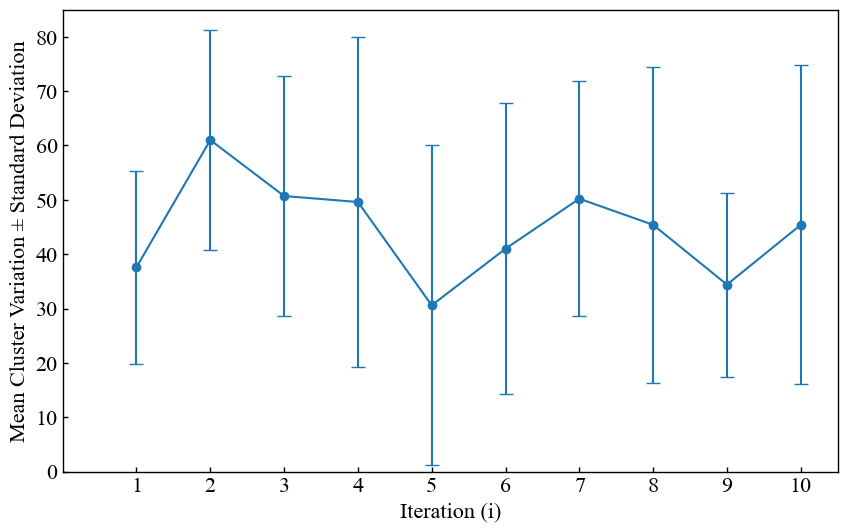
\includegraphics[width=\linewidth]{img/clustering.png}}
	\caption{Stability verification of cluster assignment for short video dataset}
	\label{fig:clustering-stability}
\end{figure}

%
Section~\ref{subsec:evaluation-short} demonstrated that three-dimensional point-cloud features are effective for activity-level estimation.
Clustering instability may partially explain the limited accuracy improvement from multiple features.
K-means clustering ($k$=3) was applied to the short-video dataset as a baseline.
One sample was randomly removed and clustering was re-run 10 times per trial, repeated over 10 trials.
Fig.~\ref{fig:clustering-stability} shows the number of changed cluster assignments.
Cluster changes ranged from approximately 20 to 40 per trial.
Clustering instability is a contributing factor to the limited accuracy improvement from multiple features.
The XGBoost all-feature model achieved the highest accuracy in Section~\ref{subsec:evaluation-short}.
The accuracy gain over single-feature models remained limited.
A baseline clustering result was established with k-means ($k$=3) on the full dataset.
Mean and standard deviation of reassignment counts were computed across 10 trials of 10 removal-and-reclustering operations.
Fig.~\ref{fig:clustering-stability} plots the mean and standard deviation on the vertical axis against trial number on the horizontal axis.


\subsubsection{Applicability to office deskwork and limitations of the evaluation scenario}
%1. 評価シナリオの限定
The evaluation used a scenario in which student participants watched SQL learning videos.
  %1-1. 付随作業
  The participants took notes during video viewing and answered a quiz afterward.
  %1-2. 被験者
  The participants were university students aged 19 to 24.
%2. 代表する動き
The scenario represents seated PC-based deskwork with small upper-body movements.
  %2-1. 制御
  Identical video content enabled controlled comparison of activity indicators and point-cloud features.
%3. 未評価のデスクワーク
Other seated deskwork in operational offices was not evaluated.
  %3-1. キーボード操作
  Sustained keyboard operation was not part of the scenario.
  %3-2. 机上会話
  Desk conversations were not part of the scenario.
%4. 適用範囲
The estimation accuracy applies to seated PC-based deskwork of the evaluated type.
  %4-1. 未検証
  Applicability to other deskwork in operational offices remains unverified.
%5. デスクワーク以外
Tasks other than seated deskwork remain outside the present estimation task.
  %5-1. 移動
  Walking to communal areas remains outside the present estimation task.
  %5-2. 機器利用
  Use of office equipment remains outside the present estimation task.


\section{Conclusion}
\label{sec:conclusion}
\deleted{We proposed an edge-computing system that estimates the activity levels of people working in office environments using a LiDAR-sensor network.  



The estimation results demonstrated that three-dimensional features derived from point-cloud data are effective for activity-level estimation.

  %

  The XGBoost model achieved its highest accuracy when all features were used as inputs.

% 

To validate the system, experiments were conducted in an office environment with multiple participants. 

% 

The collected point-cloud data were transformed into statistical features that represented different aspects of participants' movements. 

% 

To estimate activity levels, we constructed two types of machine learning models that used either single point-cloud features or all features.  

For the XGBoost model, incorporating all features achieved higher accuracy than any single-feature model.

%

For the RF model, image-based 50th percentile values achieved the highest accuracy.

%

We considered the impact of clustering instability on the estimation accuracy.}

\revised{This paper proposed the system that estimates activity levels of office workers using a LiDAR-sensor network.

Three-dimensional features derived from point-cloud data were effective for activity-level estimation.

The XGBoost model achieved the highest accuracy with all features as inputs.

The RF model achieved the highest accuracy with image-based 50th percentile values.

Clustering instability was identified as a factor limiting estimation accuracy improvement.}

\revised{Office experiments collected point-cloud data from 37 participants during SQL learning-video sessions.

Point-cloud data were converted into image-based and centroid-based statistical features.

RF and XGBoost classifiers predicted ML agreement from feature-vector differences between session pairs.}

% \begin{revisedblock}

% %1. 評価の限界

% The evaluation was limited to SQL learning-video sessions with student participants.

%   %1-1. 適用できる範囲

%   The estimation accuracy applies to seated PC-based deskwork of the evaluated type.

% %2. 未評価

% Other seated deskwork in operational offices was not evaluated.

%   %2-1. 今後

%   Future evaluation will examine other seated deskwork in operational offices.

% \end{revisedblock}



% If you have multiple appendices, use the $\backslash$appendices command below. If you have only one appendix, use
% $\backslash$appendix[Appendix Title]

\bibliographystyle{IEEEtran}
\bibliography{ref}

\input{tex/author-bibs.tex}

% \newpage
\appendix
\section{Quiz for training-dataset acquisition}
\begin{table}[h]% [!b]
  \centering
	\caption{Quiz for training-dataset acquisition}
	\begin{tabular}{cclp{3cm}} \hline
		\textbf{Video} & \textbf{No. of} & \textbf{Time} & \textbf{Content}  \\ 
		\textbf{no.} & \textbf{Items} & \textbf{(Seconds)} &  \\ \hline
		1 & 5 & 300 & Basic knowledge quiz about SQL platforms and tools		\\
		2 & 5 & 300 & Understanding quiz about SQL basic operations and data types \\ 
		3 & 5 & 300 & Understanding quiz about SQL table creation and data types \\
		% 4 & 7 & 300 & Test on SQL query operations and data management \\
		\hline
	\end{tabular}
	\label{quiz_train}
\end{table}

% \begin{table}[!b]
%   \centering
% 	\caption{Questionnaire for training-dataset acquisition}
% 	\begin{tabular}{cclp{3cm}} \hline
% 		\textbf{Video} & \textbf{No. of} & \textbf{Content}  \\ 
% 		\textbf{no.} & \textbf{Items} &  \\ \hline 
% 		1,2,3,4 & 3 & Video content comprehension surveys	\\ \hline
% 	\end{tabular}
% 	\label{questionnaire_train}
% \end{table}

% \begin{table}[!b]
%   \centering
% 	\caption{Quiz for test-dataset acquisition}
% 	\begin{tabular}{cclp{3cm}} \hline
% 		\textbf{Video} & \textbf{No. of} & \textbf{Time} & \textbf{Content}  \\ 
% 		\textbf{no.} & \textbf{Items} & \textbf{(Seconds)} &  \\ \hline
% 		1 & 10 & 600 & Comprehensive Test on SQL Query Operations and Table Management \\ \hline
% 	\end{tabular}
% 	\label{quiz_test}
% \end{table}

% \begin{table}[!b]
%   \centering
% 	\caption{Questionnaire for test-dataset acquisition}
% 	\begin{tabular}{cclp{3cm}} \hline
% 		\textbf{Video} & \textbf{No. of} & \textbf{Content}  \\ 
% 		\textbf{no.} & \textbf{Items} &  \\ \hline 
% 		1 & 3 & Video content comprehension surveys	\\ \hline
% 	\end{tabular}
% 	\label{questionnaire_test}
% \end{table}

\EOD

\end{document}
